\documentclass[
    12pt,
    openright,
    twoside,
    a4paper,
    english,
    spanish,
    brazil,
    ]{abntex2}

% ---
% PACOTES
% ---

\usepackage{cmap}
\usepackage{lmodern}
\usepackage[T1]{fontenc}
\usepackage[utf8]{inputenc}
\usepackage{lastpage}
\usepackage{indentfirst}
\usepackage{color}
\usepackage{graphicx}
\usepackage{lipsum}
\usepackage[brazilian,hyperpageref]{backref}
\usepackage[alf]{abntex2cite}
\usepackage[table,xcdraw]{xcolor}

\renewcommand{\backrefpagesname}{Citado na(s) página(s):~}
\renewcommand{\backref}{}
\renewcommand*{\backrefalt}[4]{
    \ifcase #1 %
        Nenhuma citação no texto.%
    \or
        Citado na página #2.%
    \else
        Citado #1 vezes nas páginas #2.%
    \fi}%
% ---


% ---
% Informações de dados para CAPA e FOLHA DE ROSTO
% ---
\titulo{Protótipo de sistema embutido de baixo custo integrado ao Amazon Voice Service}
\autor{Guilherme Vinícius Barbosa Pereira Amorim}
\local{Belo Horizonte}
\data{2022}
\orientador{Prof. Ricardo de Oliveira Duarte}
%\coorientador{Prof. }
\instituicao{%
  Universidade Federal de Minas Gerais -- UFMG
  \par
  Escola de Engenharia
  \par
  Curso de Graduação em Engenharia Elétrica}
\tipotrabalho{Trabalho de Conclusão de Curso}

% O preambulo deve conter o tipo do trabalho, o objetivo, o nome da instituição e a área de concentração
\preambulo{Monografia apresentada durante o Seminário dos Trabalhos de Conclusão do Curso de Graduação em Engenharia Elétrica da UFMG, como parte dos requisitos necessários à obtenção do título de Engenheiro Eletricista.}
% ---

% ---
% Configurações de aparência do PDF final

% alterando o aspecto da cor azul
\definecolor{blue}{RGB}{41,5,195}

% informações do PDF
\makeatletter
\hypersetup{
         %pagebackref=true,
        pdftitle={\@title},
        pdfauthor={\@author},
        pdfsubject={\imprimirpreambulo},
        pdfcreator={LaTeX with abnTeX2},
        pdfkeywords={abnt}{latex}{abntex}{abntex2}{trabalho acadêmico},
        colorlinks=true,
        linkcolor=blue,
        citecolor=blue,
        filecolor=magenta,
        urlcolor=blue,
        bookmarksdepth=4
}
\makeatother
% ---

% ---
% Espaçamentos entre linhas e parágrafos
% ---

% O tamanho do parágrafo é dado por:
\setlength{\parindent}{1.3cm}

% Controle do espaçamento entre um parágrafo e outro:
\setlength{\parskip}{0.2cm}

% ---
% compila o índice
% ---
\makeindex
% ---

% ----
% Início do documento
% ----
\begin{document}

% Retira espaço extra obsoleto entre as frases.
\frenchspacing

% ----------------------------------------------------------
% ELEMENTOS PRÉ-TEXTUAIS
% ----------------------------------------------------------
% \pretextual

% ---
% Capa
% ---
\imprimircapa
% ---

% ---
% Folha de rosto
% ---
\imprimirfolhaderosto
% ---

% ---
% Dedicatória
% ---
\begin{dedicatoria}
\end{dedicatoria}
% ---

% ---
% Agradecimentos
% ---
\begin{agradecimentos}
\end{agradecimentos}
% ---

% ---
% inserir o sumario
% ---
\pdfbookmark[0]{\contentsname}{toc}
\tableofcontents*
\cleardoublepage
% ---

% ----------------------------------------------------------
% ELEMENTOS TEXTUAIS
% ----------------------------------------------------------
\textual

% ----------------------------------------------------------
% Capítulo 1 - Introdução
% ----------------------------------------------------------
\chapter{Introdução}
Atualmente o termo ‘sistemas embarcados’ não está muito presente no cotidiano brasileiro, mas essa tecnologia é responsável por fornecer equipamentos inteligentes como semáforos de trânsito, relógios, respiradores mecânicos, roteadores e aparelhos de ar-condicionado, por exemplo. Em termos simples, pode-se definir um sistema embarcado como um dispositivo controlado por um computador encapsulado. Ou seja, um sistema embarcado é na verdade um sistema microprocessado. Dentre as principais vantagens de sistemas embarcados, destaca-se o baixo custo, a eficiência e a facilidade de programação (NORLETO, 2020).

O primeiro sistema embarcado é o AGC (Apollo Guidance Computer). Ele foi desenvolvido nos EUA por Charles Stark Draper do MIT em 1966 (EMBARCADOS, 2014). Desde então, os sistemas embarcados ficaram mais acessíveis, mais velozes e mais compactos.

Com o passar dos anos, novas tecnologias foram adicionadas à sistemas embarcados, como por exemplo o Wifi, o Bluetooth etc. Na última década foi observado a ascensão de assistentes virtuais como a Alexa e o Google Assistente. A Alexa foi criada em 2014 e apareceu pela primeira vez como parte das caixas de som. Hoje a Alexa, a partir de comandos de voz, pode realizar pesquisas, mandar executar uma lista de músicas, disparar um alarme etc (VIGLIAROLO, 2017). Segundo o site oficial da Amazon Alexa (2022), o serviço permite a conexão com dispositivos, efetuar comandos por voz, interpretá-los e tomar uma ação correspondente. Isso tudo acontece por meio do Web Service da Amazon (AWS).

Em 25 de setembro de 2019, o Alexa e o Google Assistant puderam ajudar seus usuários a se candidatarem a empregos no McDonald's usando serviços de reconhecimento de voz. É o primeiro serviço de emprego do mundo usando o serviço de comando de voz. A Amazon anunciou em 25 de setembro de 2019 que Alexa em breve poderá imitar vozes de celebridades, incluindo Samuel L. Jackson, custando US \$ 0,99 para cada voz.

Visto que as tecnologias Amazon AWS e Amazon Alexa são recente, ainda não se observa uma variedade de dispositivos, não comercializados pela Amazon e pela Google, que fazem o uso de linguagem natural. Com a baixa oferta de produtos com essa tecnologia, produtos simples - como interruptores - estão sendo comercializados por preços não acessíveis ao mercado global.

Diante do que foi dito, este trabalho se propõe criar um dispositivo de baixo custo integrado à tecnologia AVS e serviços em nuvem.

\section{Estrutura}
O trabalho será apresentado em cinco capítulos. O capítulo 1 apresenta a introdução e os objetivos. O capítulo 2 apresenta o referencial teórico, contextualizando o projeto e citando trabalhos correlatos. O capítulo 3 contém o desenvolvimento do trabalho, apresentando requisitos funcionais e não-funcionais, ferramentas utilizadas e a implementação. O capítulo 4 expõe e faz a análise dos resultados. O capítulo 5, por fim, conclui o trabalho listando vantagens e desvantagens do protótipo, e as sugestões para trabalhos futuros.

% ----------------------------------------------------------
% Capítulo 2 - Referencial teórico
% ----------------------------------------------------------
\chapter{Referencial teórico}


% ----------------------------------------------------------
% Capítulo 2.1 - IoT
% ----------------------------------------------------------
\section{IoT}
Nos últimos anos, observou-se a ascensão de dispositivos inteligentes, dispositivos que se conectam à Internet. Esses dispositivos se comunicam entre si, possuem sensores, softwares e outras tecnologias. Essa rede de dispositivos, softwares, sensores etc descreve o que denominamos internet das coisas, ou IoT. Define-se IoT como uma rede que engloba um sistema de dispositivos de computação inter-relacionados, máquinas mecânicas e digitais, objetos, animais ou pessoa, e a capacidade de transferir dados através de uma rede sem a necessidade de interação entre humanos (Alexander S. Gillis, 2022). A presença de tecnologias de nuvem, \textit{big data} e redes móveis, por exemplo, em redes de IoT permite o compartilhamento e a coleta de dados com o mínimo de intervenção humana (ORACLE, 2022). Pode-se listar as seguintes tecnologias como as protagonistas no crescimento do uso da tecnologia IoT:
\begin{itemize}
	\item Acesso a tecnologia de sensores de baixo custo e baixa potência;
	\item Conectividade;
	\item Plataformas de computação em nuvem;
	\item Machine learning e análise avançada;
	\item Processamento de linguagem natural (AVS, por exemplo).
\end{itemize}

Uma característica comum dos dispositivos IoT é a necessidade de componentes de interface para a interação com o mundo físico. Alguns exemplos de componentes de interface são:
\begin{itemize}
	\item Teclado, botões e microfones;
	\item Alarmes, visores e alto-falantes;
	\item Sensores;
	\item Atuadores;
\end{itemize}

% ----------------------------------------------------------
% Capítulo 2.2 - Computação em nuvem com a AWS
% ----------------------------------------------------------
\section{Computação em nuvem com a AWS}
A Amazon Web Services, Inc. (AWS) é uma empresa subsidiária da Amazon responsável por fornecer a seus clientes plataformas para a computação em nuvem sob demanda via Internet. Empresas fazem uso desse serviço para a criação e execução de aplicações virtuais sem um custo inicial, uma vez que a AWS tem o \textit{pay-as-you-go} como modelo de precificação. Ou seja, o cliente faz o pagamento conforme o uso (AWS, 2019). Em 2022, a AWS é capaz de oferecer a seus clientes mais de duzentos serviços em nuvem nas áreas de tecnologias de computação, banco de dados, \textit{machine learning}, IoT, inteligência artificial etc.

Ademais, a AWS conta com 84 zonas de disponibilidade em 26 regiões geográficas. Esse modelo de região e zona de disponibilidade da AWS foi reconhecido pelo Gartner, empresa de pesquisa e consultoria em tecnologia da informação (TI), como o método recomendado para executar aplicativos corporativos que exigem alta disponibilidade (AWS, 2022). As \autoref{fig_aws_zone} contém mapas com as redes de presença da AWS, por região.

\begin{figure}[htb]
	\caption{AWS Presence Networks.}\label{fig_aws_zone}
	\begin{center}
		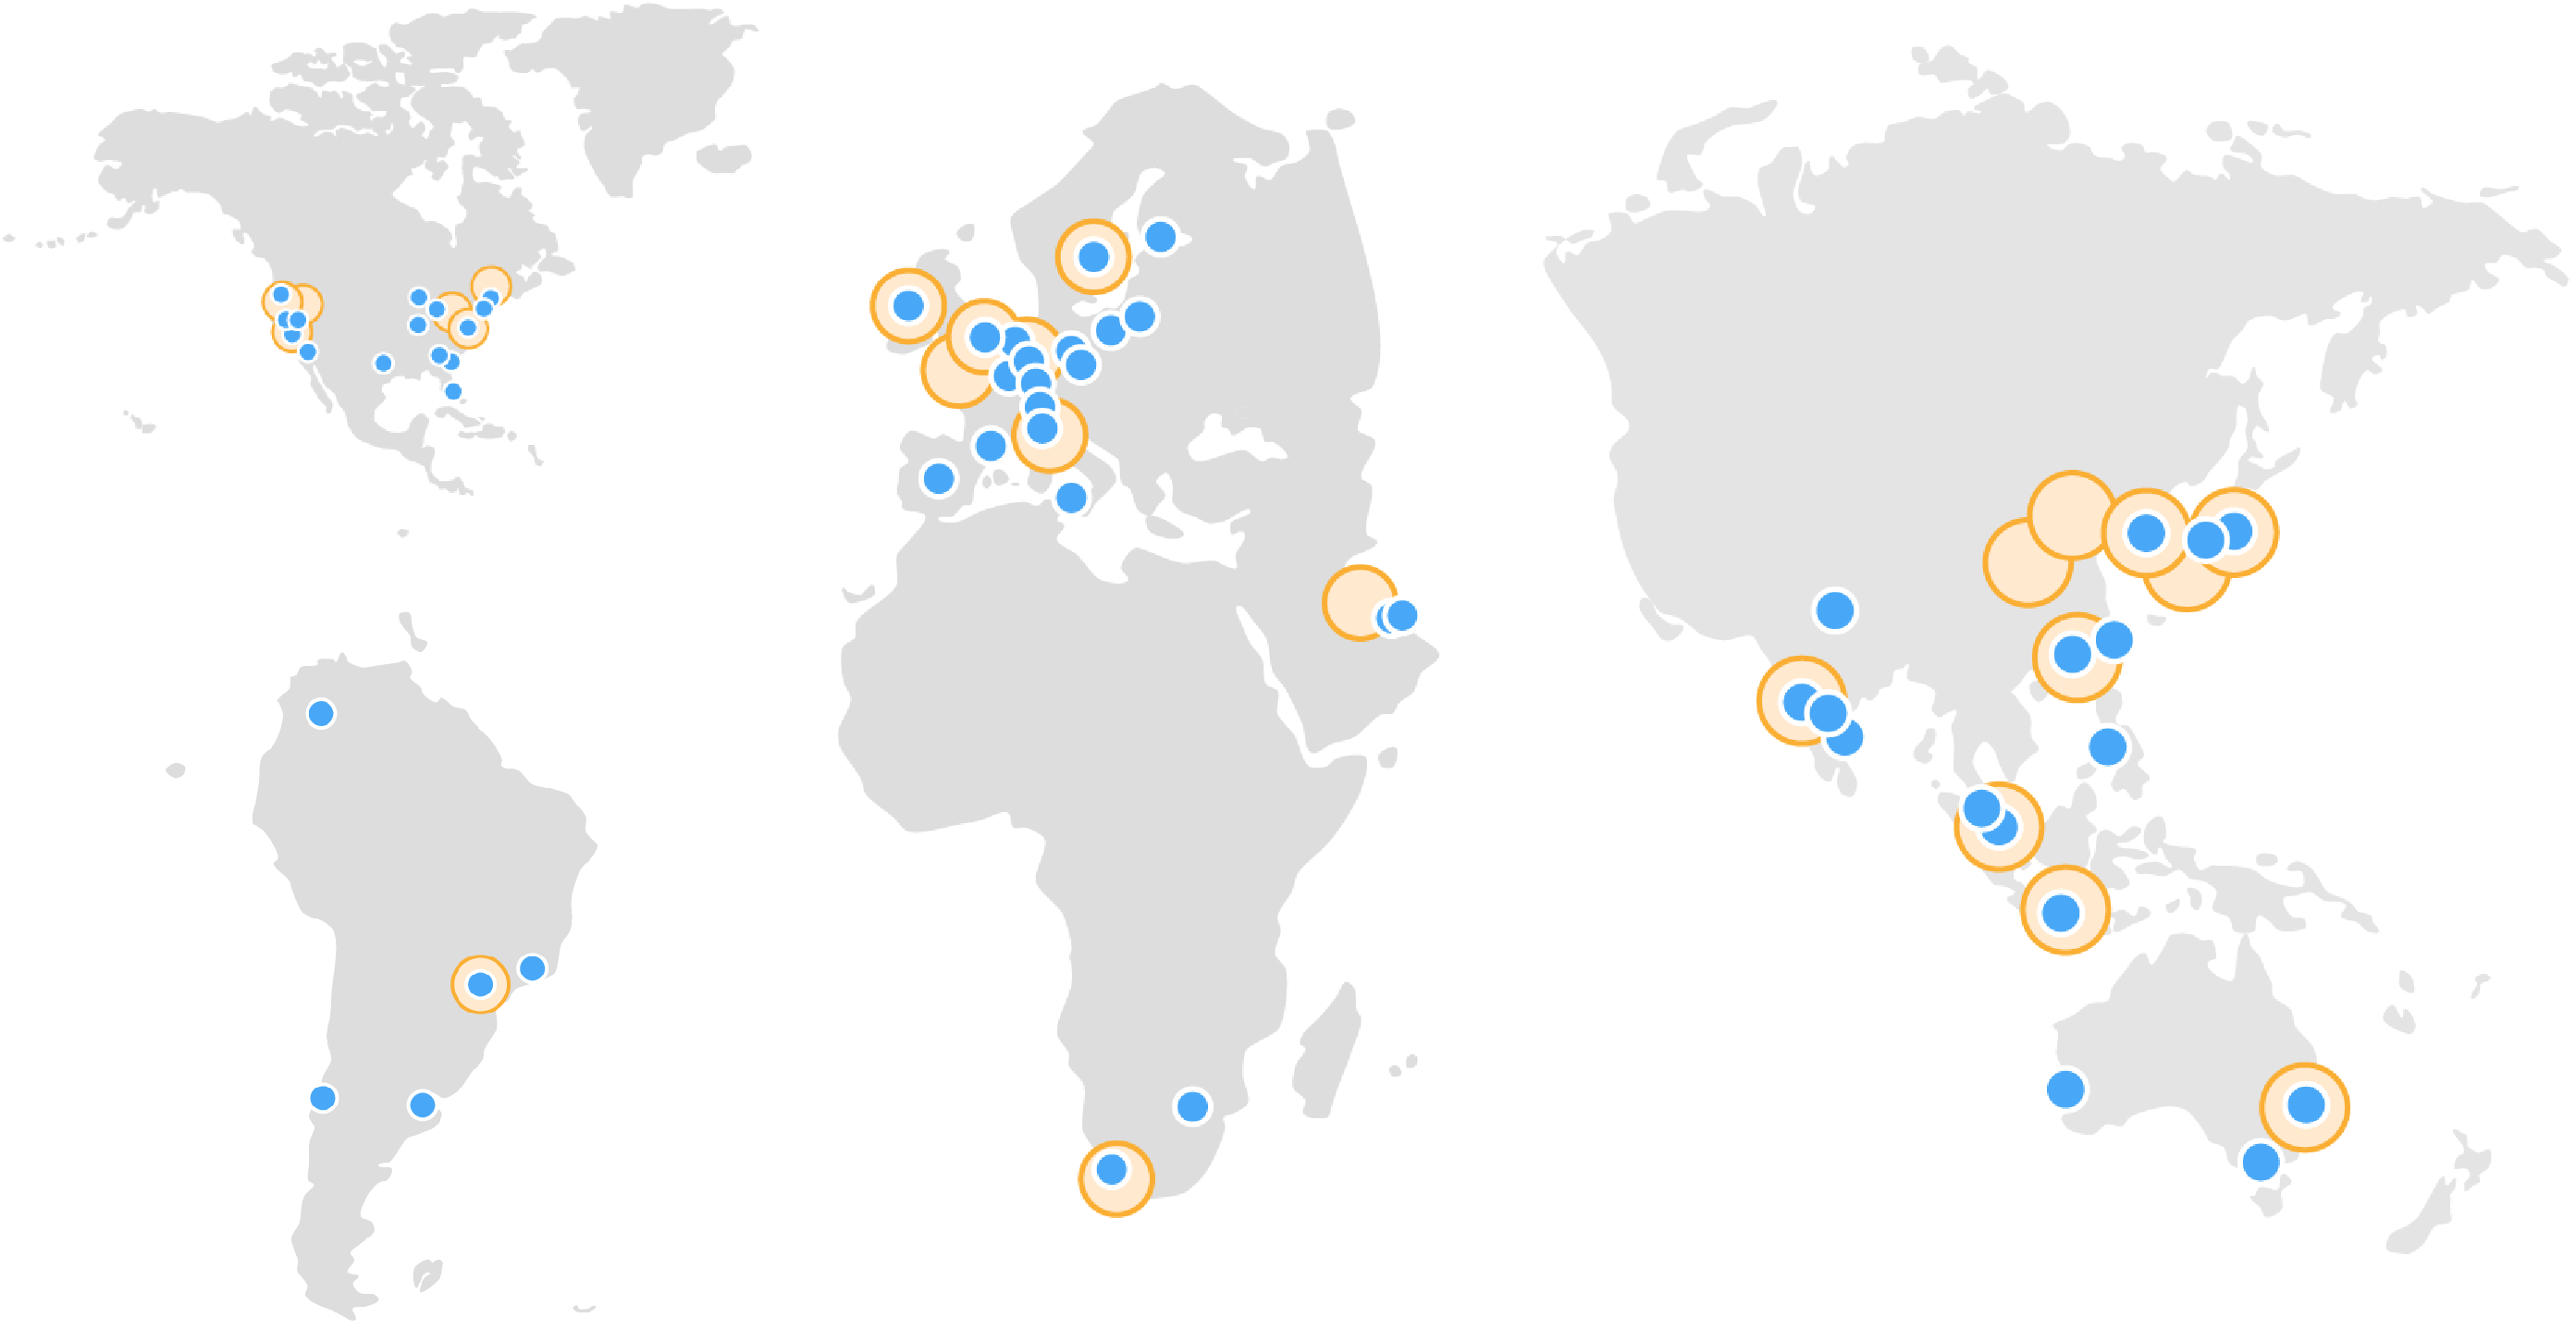
\includegraphics[scale=0.3]{Images/aws_zones.pdf}
		\legend{Fonte: Author.}
	\end{center}
\end{figure}

Para o desenvolvimento de aplicações na AWS, a Amazon oferece ao desenvolvedor ferramentas e permite a escolha da linguagem de programação. Destaca-se as seguintes ferramentas:
\begin{itemize}
	\item Console da web;
	\item Ferramenta de linha de comando;
	\item Ambiente de desenvolvimento integrado (IDE);
	\item Kit de desenvolvimento de software (SDK);
	\item Infraestrutura como código.
\end{itemize}


% ----------------------------------------------------------
% Capítulo 2.3 - AWS IoT
% ----------------------------------------------------------
\section{AWS IoT}

O AWS IoT é um conjunto de serviços em nuvem oferecidos pela AWS que permitem a conexão de dispositivos IoT a outros dispositivos e a outros serviços oferecidos pelo AWS. Em termos simples, o AWS IoT funciona como uma ponte entre dispositivos IoT e os serviços em nuvem que a AWS fornece, assim como pode ser visto na \autoref{fig_what_is_iot}.

\begin{figure}[htb]
	\caption{Integração de dispositivos IoT com serviços AWS por meio do AWS IoT.}\label{fig_what_is_iot}
	\begin{center}
		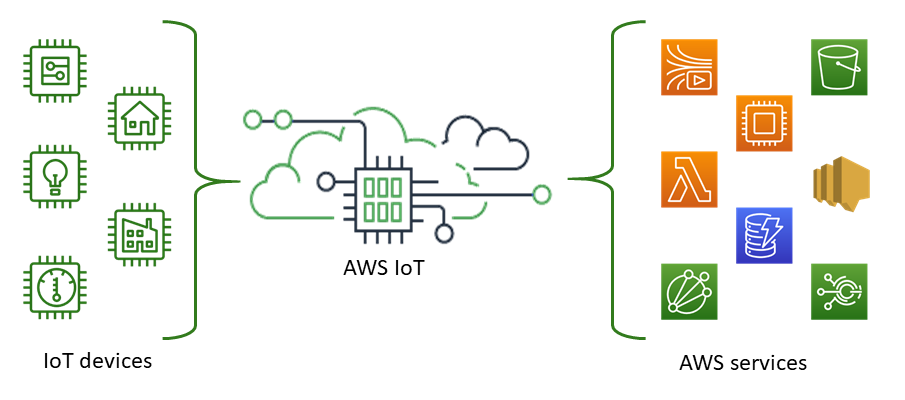
\includegraphics[scale=0.5]{Images/what-is-aws-iot.png}
		\legend{Fonte: Amazon AWS (2022).}
	\end{center}
\end{figure}

Os dispositivos IoT geralmente estão localizados próximos às interfaces do mundo real que monitoram e/ou controlam. Eles geralmente também incluem recursos de computação e armazenamento, como microcontroladores, CPUs e memórias. Alguns exemplos de dispositivos disponíveis no mercado são:
\begin{itemize}
	\item LoRaWAN e dispositivos;
	\item Arduino;
	\item Raspberry PI;
	\item Dispositivos de IoT personalizados.
\end{itemize}

Para a completa integração desses dispositivos com serviços AWS e usuários, alguns componentes são esseciais. Aplicativos de celulares, por exemplo, são utilizados para que o usuário tenha acesso aos seus aparelhos e os configure conforme a sua preferência. Tem-se como outro exemplo os protocolos utilizados para a comunicação dos dispositivos com serviços em nuvem. A tecnologia AWS IoT possui suporte para os seguintes protocolos:
\begin{itemize}
	\item MQTT;
	\item HTTPS;
	\item LoRaWAN.
\end{itemize}

O protocolo MQTT será melhor detalhado na sessão \autoref{section_mqtt}. Para o desenvolvimento de softwares a nível de dispositivo, o AWS IoT também fornece suporte para um sistema operacional em tempo real para microcontroladores, o FreeRTOS, que será melhor detalhado na sessão \autoref{section_free_rtos}. Alguns exemplos de outros serviços fornecidos pelo AWS IoT podem ser vistos na \autoref{fig_aws_iot_architecture}.

\begin{figure}[htb]
	\caption{AWS IoT architecture.}\label{fig_aws_iot_architecture}
	\begin{center}
		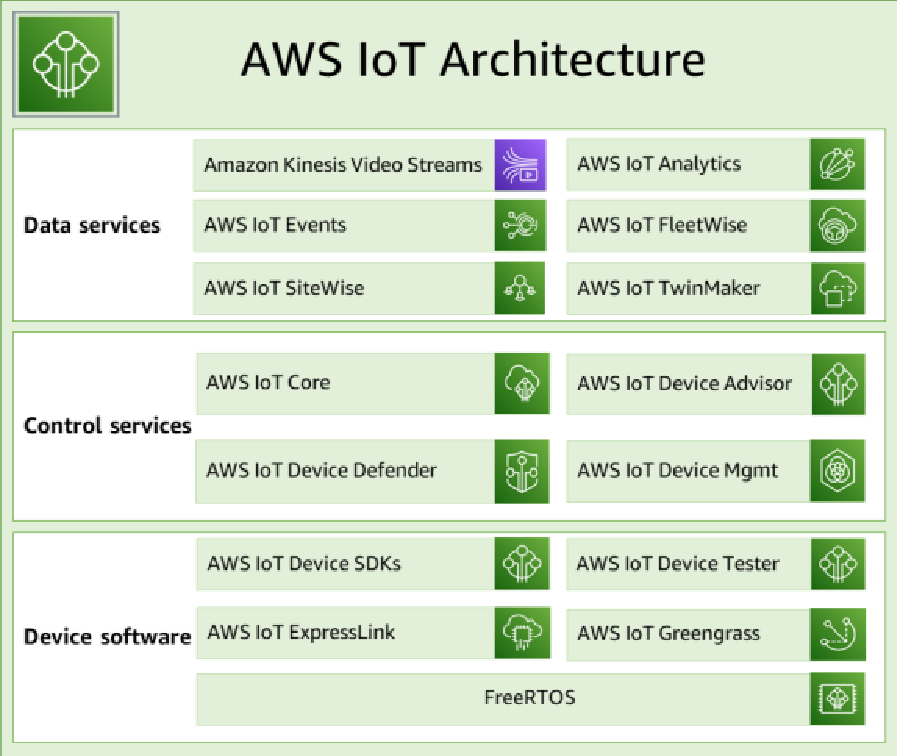
\includegraphics[scale=0.7]{Images/aws_iot_architecture.pdf}
		\legend{Fonte: AWS IoT Core - Guia do desenvolvedor (2022).}
	\end{center}
\end{figure}

O serviço IoT Core será melhor detalhado na sessão \autoref{section_aws_iot_core}.
a
% ----------------------------------------------------------
% Capítulo 2.4 - Amazon FreeRTOS
% ----------------------------------------------------------
\section{Amazon FreeRTOS}\label{section_free_rtos}
O FreeRTOS é um kernel de sistema operacional em tempo real de código aberto para microcontroladores e distribuído sob a licença do MIT. O seu logo pode ser visto na \autoref{fig_logo_free_rtos}. Originalmente, o FreeRTOS foi desenvolvido em 2003 por Richard Barry e posteriormente mantido pela empresa Real Time Engineers Ltd. Em 2017, a AWS assumiu a administração do kernel. Além de ser um kernel de código aberto, a distribuição do FreeRTOS conta com demonstrações e documentação para diferentes compiladores. Essas características permitem um rápido desenvolvimento dispositivos.

\begin{figure}[htb]
	\caption{Logo FreeRTOS.}\label{fig_logo_free_rtos}
	\begin{center}
		
\includegraphics[scale=1.5]{Images/Logo_freeRTOS.png}
		\legend{Fonte: Wikipedia (2022).}
	\end{center}
\end{figure}

O FreeRTOS surgiu com o propósito de ser simples, compacto, ágil e com baixo consumo de energia. Essa característica o torna o kernel escolhido por diversos dispositivos de IoT. Sua estrutura é baseada em uma arquitetura de rotinas programáveis (\textit{scheduler routines}). Ele também é capaz de fazer alocações de memória estaticamente e/ou dinamicamente. Atualmente, o FreeRTOS conta com métodos que possibilitam a implementação dos seguintes componentes e \textit{features}:
\begin{alineas}
	\item \textit{Threads};
	\item \textit{tasks} e suporte para \textit{Coroutines};
	\item Priorização de \textit{Threads};
	\item Mutexes;
	\item Semáforos;
	\item \textit{timers};
	\item O \textit{scheduler} pode ser configurado para \textit{preemptive} ou \textit{cooperative multitasking};
	\item modo \textit{tickless}, para aplicações de baixo consumo;
	\item Visualizador em tempo de tempo de execução para depuração e verificação.
\end{alineas}

Em 2022, mais de 90 microcontroladores estão disponíveis no mercado para o desenvolvimento de aplicações baseadas no FreeRTOS. A AWS conta hoje com verificador que permite que o usuário confirme se algum dispositivo é compatível com o seu kernel, o \textit{AWS IoT Device Tester}. Isso possibilita que usuários e empresas testem, inclusive, microcontroladores não disponíveis no mercado. Esse verificador faz uso do do AWS IoT Core, serviço que será melhor explicado na \autoref{section_aws_iot_core}. A \autoref{fig_aws_iot_device_tester} mostra o diagrama de conexões para o \textit{AWS IoT Device Tester}. Ademais, a AWS também disponibiliza um simulador do FreeRTOS para Windows que possibilita o teste de software sem hardware.

\begin{figure}[htb]
	\caption{Diagrama de conexões para o \textit{AWS IoT Device Tester}.}\label{fig_aws_iot_device_tester}
	\begin{center}
		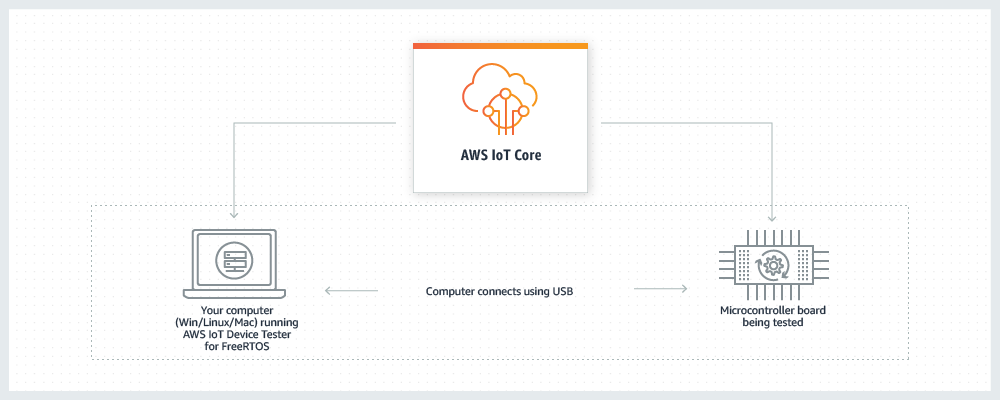
\includegraphics[scale=0.4]{Images/aws_iot_device_tester.png}
		\legend{Fonte: Amazon AWS (2022).}
	\end{center}
\end{figure}

Durante o processo de desenvolvimento, as bibliotecas necessárias para o projeto podem ser obtidas no próprio site da AWS, GitHub ou FreeRTOS.org. Também é possível acessar o kernel FreeRTOS autônomo por meio de qualquer um desses canais. Vale lembrar que o FreeRTOS tem código aberto, portanto, o desenvolvedor pode ampliar, modificar ou excluir qualquer uma das bibliotecas de código-fonte. O processo de download personalizado das bibliotecas é orientado por console e interface gráfica na AWS. Um fluxo recomendado pela AWS para o \textit{deploy} de dispositivos usando o FreeRTOS pode ser visto na \autoref{fig_iot_devide_deploy}.
\begin{figure}[htb]
	\caption{Fluxo recomendado pela AWS para o \textit{deploy} de dispositivos usando o FreeRTOS.}\label{fig_iot_devide_deploy}
	\begin{center}
		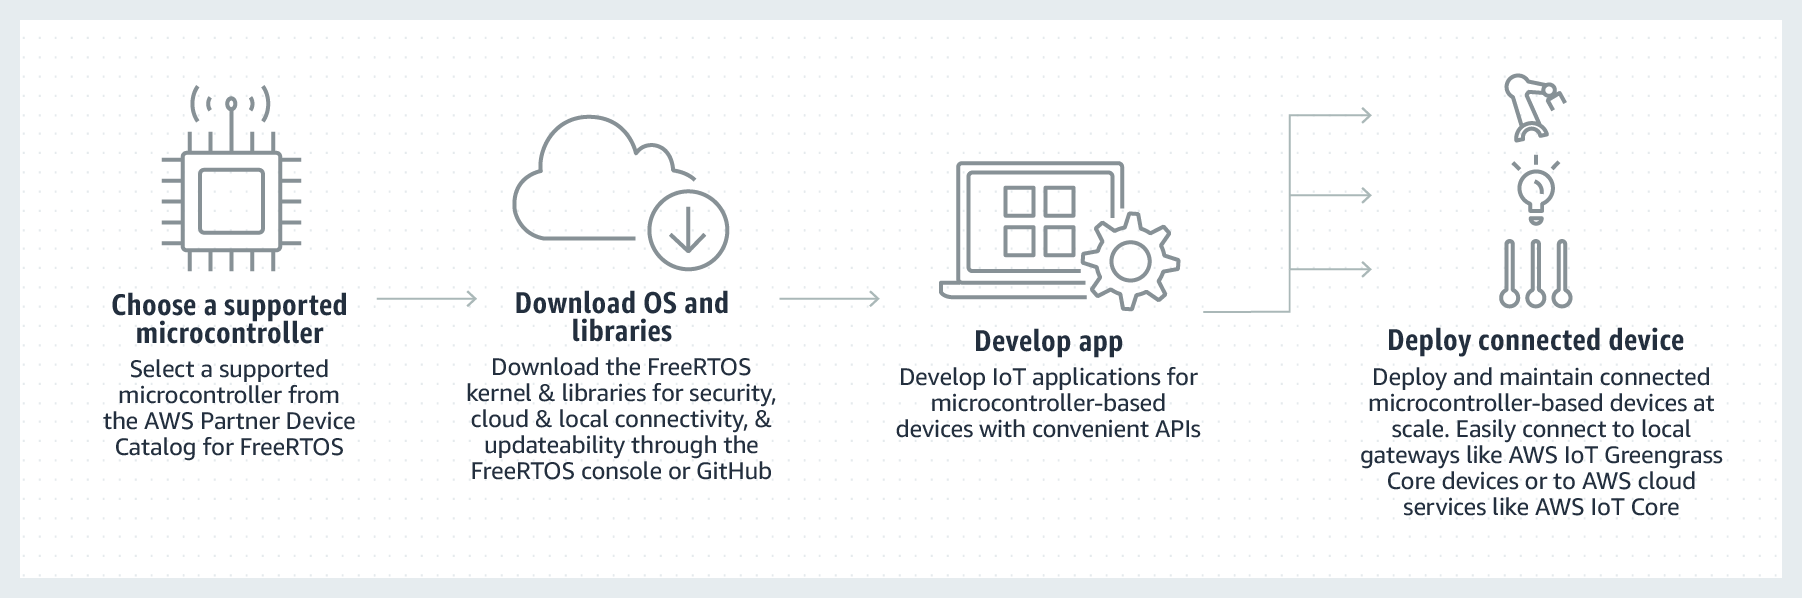
\includegraphics[scale=0.4]{Images/iot_device_deploy.png}
		\legend{Fonte: Amazon AWS (2022).}
	\end{center}
\end{figure}

% ----------------------------------------------------------
% Capítulo 2.5 - AWS IoT Core
% ----------------------------------------------------------
\section{AWS IoT Core}\label{section_aws_iot_core}
O AWS IoT Core é serviço de controle oferecido pela AWS que permite a conexão de bilhões de dispositivos de IoT e rotear trilhões de mensagens para serviços da AWS sem que o usuário tenha que gerenciar a infraestrutura. Esse serviço está disponível gratuitamente para clientes por doze meses a partir da data em que a conta da AWS é criada. Haverá taxas de uso do AWS IoT core após doze meses de uso ou quando a aplicação exceder os níveis de uso gratuito descritos abaixo:
\begin{itemize}
	\item 2.250.000 minutos de conexão;
	\item 500.000 mensagens;
	\item 225.000 operações do Registry ou Device Shadow;
	\item 250.000 regras acionadas e 250.000 ações executadas.
\end{itemize}

Dessa forma, o AWS IoT Core é o serviço que permite a integração da AVS à sistemas embarcados. Essa integração acontece via protocolo MQTT. Os preços cobrados pela AWS após doze meses de uso ou excedendo os limites já citados pode ser visto abaixo:
\begin{itemize}
	\item Preço da conectividade: 0,12 USD (por milhão de minutos de conexão);
	\item Até 1 bilhão de mensagens MQTT e HTTP: 1,50 USD (por milhão de mensagens);
	\item Próximos 4 bilhões de mensagens MQTT e HTTP: 1,20 USD (por milhão de mensagens);
	\item Mais de 5 bilhões de mensagens MQTT e HTTP: 1,05 USD (por milhão de mensagens).
\end{itemize}

A \autoref{fig_aws_iot_core_integrated_alexa} mostra um diagrama disponibilizado pela AWS que melhor apresenta como o AWS IoT Core permite a integração de sistemas embutidos à AVS:
\begin{figure}[htb]
	\caption{Diagrama de integração de sistemas embutidos à AVS por meio do AWS IoT Core.}\label{fig_aws_iot_core_integrated_alexa}
	\begin{center}
		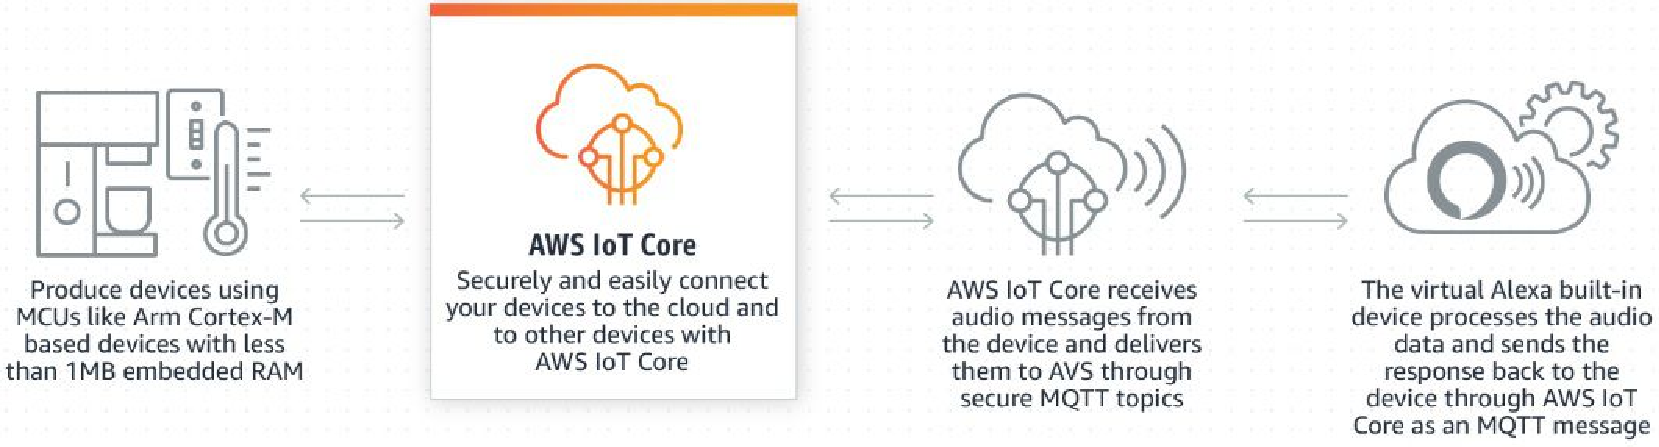
\includegraphics[scale=0.5]{Images/aws_iot_core_integrated_alexa.pdf}
		\legend{Fonte: Amazon AWS (2022).}
	\end{center}
\end{figure}

% ----------------------------------------------------------
% Capítulo 2.6 - MQTT
% ----------------------------------------------------------
\section{MQTT}\label{section_mqtt}
MQTT é um protocolo de mensagens para dispositivos IoT. Ele foi desenvolvido para dispositivos com limitada disponibilidade de largura de banda (\textit{network bandwidth}). Ele deve ser executado em um protocolo de transporte que forneça conexões bidirecionais ordenadas, sem perdas — normalmente, TCP/IP. O logo do MQTT pode ser visto na \autoref{fig_logo_mqtt}.
\begin{figure}[htb]
	\caption{Logo MQTT.}\label{fig_logo_mqtt}
	\begin{center}
		
\includegraphics[scale=0.3]{Images/logo_mqtt.pdf}
		\legend{Fonte: Wikimedia (2022).}
	\end{center}
\end{figure}

No protocolo MQTT, existem dois tipos de entidades: o \textit{message broker} e os clientes. Um \textit{message broker} é um servidor que tem o papel de receber diversas mensagens dos diversos clientes e, então, as rotear para os clientes de destino. Já um cliente pode ser qualquer dispositivo que se comunica via rede com o \textit{message broker}, a partir de bibliotecas do protocolo MQTT.

As informações são organizadas em hierarquia de tópicos. Quando algum cliente possui um novo item de dados para distribuir, ele envia uma mensagem de controle com os dados para o \textit{message broker}. O \textit{broker}, então, distribui as informações para todos os clientes que se inscreveram nesse tópico. O cliente remetente (\textit{publisher}) não precisa ter nenhuma informação sobre número de clientes que irão receber essa mensagem. Os clientes destinatários, por sua vez, também não precisam ser configurados com nenhuma informação dos destinatários.

Os sete tipos de mensagens existentes no protocolo MQTT são:
\begin{itemize}
	\item \textit{Connect}: Aguarda o estabelecimento de uma conexão com o \textit{message broker} e cria um link entre os nós;
	\item \textit{Disconnect}: Aguarda o fim da tarefa que está sendo executada pelo cliente e desconecta a sessão TCP/IP;
	\item \textit{Publish}: Mensagem a ser distribuída para os clientes inscritos. Mais informações sobre esse tipo de mensagem pode ser encontrado na \autoref{section_mqtt_publish_message}.
	\item \textit{Subscribe}: Para receber mensagens sobre tópicos de interesse, o cliente envia uma mensagem \textit{Subscribe} para o \textit{broker}. Mais informações sobre esse tipo de mensagem pode ser encontrado na \autoref{section_mqtt_subscribe_message};
	\item \textit{Suback}: Para confirmar cada assinatura, o \textit{broker} envia uma mensagem de confirmação \textit{Suback} ao cliente. Mais informações sobre esse tipo de mensagem pode ser encontrado na \autoref{section_mqtt_subscribe_message};
	\item \textit{Unsubscribe}: Esta mensagem exclui as assinaturas existentes de um cliente no \textit{broker}. Mais informações sobre esse tipo de mensagem pode ser encontrado na \autoref{section_mqtt_unsubscribe_message};
	\item \textit{Unsuback}: Para confirmar o cancelamento de assinatura, o \textit{broker} envia uma mensagem de confirmação \textit{Unsuback} ao cliente. Mais informações sobre esse tipo de mensagem pode ser encontrado na \autoref{section_mqtt_unsuback_message}.
\end{itemize}

Depois que um cliente envia com êxito a mensagem \textit{Subscribe} e recebe a mensagem \textit{Suback}, ele obtém todas as mensagens publicadas de um tópico nas assinaturas contidas da mensagem \textit{Subscribe}. Após receber o \textit{Unsuback} do \textit{broker}, o cliente pode assumir que as assinaturas na mensagem \textit{Unsubscribe} foram excluídas.

Se o \textit{message broker} receber uma mensagem em um tópico para o qual não há assinantes, a mensagem será descartada. Quando um cliente \textit{publisher} se conecta pela primeira vez ao \textit{broker}, ele pode configurar uma mensagem padrão para ser enviada aos assinantes se o \textit{broker} detectar que o cliente \textit{publisher} se desconectou inesperadamente.

Os clientes interagem apenas com um \textit{broker}, mas um sistema pode conter vários \textit{brokers} que trocam informações com base nos tópicos de seus assinantes atuais. Uma mensagem de controle MQTT deve ter entre dois e duzentos e cinquenta e seis bytes. O MQTT conta com o protocolo TCP para transmissão de dados. Uma variante, MQTT-SN, é usada com outros protocolos de transporte, como UDP ou Bluetooth.

% ----------------------------------------------------------
% Capítulo 2.6.1 - MQTT Publish Message
% ----------------------------------------------------------
\subsection{MQTT Publish Message}\label{section_mqtt_publish_message}
O formato de uma mensagem do tipo \textit{Publish} está apresentado na \autoref{fig_mqtt_publish_message_attributes}.
\begin{figure}[htb]
	\begin{center}
		\caption{Atributos de uma mensagem do tipo \textit{Publish} para o protocolo MQTT.}\label{fig_mqtt_publish_message_attributes}
		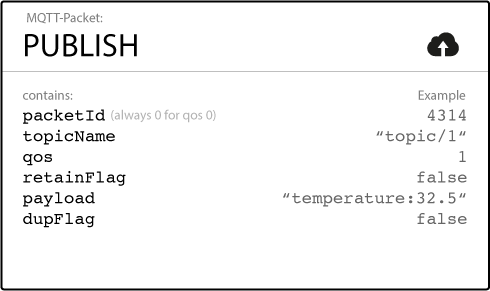
\includegraphics[scale=0.5]{Images/mqtt_publish_message_attributes.png}
	\end{center}
	\legend{Fonte: HiveMQ (2015).}
\end{figure}

Os atributos de uma mensagem do tipo \textit{Publish} são caracterizados abaixo:
\begin{itemize}
	\item packetId: O identificador de pacote identifica exclusivamente uma mensagem;
	\item topicName: O nome do tópico é uma \textit{string} simples que é estruturada hierarquicamente com barras como delimitadores (“alexa/builtin/device”, por exemplo);
	\item qos: Indica o nível de qualidade de serviço (QoS) da mensagem. Existem três níveis: 0, 1 e 2. O nível de serviço determina que tipo de garantia uma mensagem tem para chegar ao destinatário pretendido (cliente ou \textit{broker}).
	\item retainFlag: Sinalizador indicando se a mensagem é salva pelo \textit{broker} como o último valor válido conhecido para um tópico especificado. Quando um novo cliente se inscreve em um tópico, ele recebe a última mensagem retida nesse tópico.
	\item payLoad: Conteúdo  da mensagem. O MQTT é \textit{data-agnostic}. Ou seja, é possível enviar qualquer tipo de informação que pode ser codificada em formato binário.
	\item dupFlag: Indica se a mensagem é uma duplicata e foi reenviada porque o destinatário pretendido (cliente ou \textit{broker}) não enviou uma resposta de \textit{acknowledge}.
\end{itemize}

% ----------------------------------------------------------
% Capítulo 2.6.2 - MQTT Subscribe Message
% ----------------------------------------------------------
\subsection{MQTT Subscribe Message}\label{section_mqtt_subscribe_message}
O formato de uma mensagem do tipo \textit{Subscribe} está apresentado na \autoref{fig_mqtt_subscribe_message_attributes}. Esta mensagem de assinatura é muito simples, contém um identificador de pacote exclusivo e uma lista de assinaturas.
\begin{figure}[htb]
	\begin{center}
		\caption{Atributos de uma mensagem do tipo \textit{Subscribe} para o protocolo MQTT.}\label{fig_mqtt_subscribe_message_attributes}
		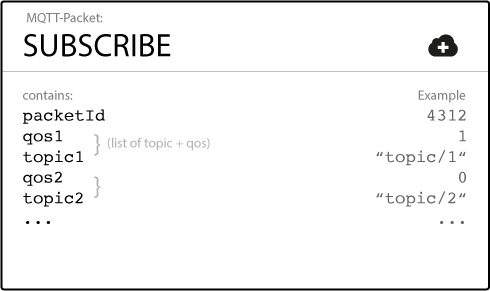
\includegraphics[scale=0.5]{Images/mqtt_subscribe_message_attributes.png}
	\end{center}
	\legend{Fonte: HiveMQ (2015).}
\end{figure}

Os atributos de uma mensagem do tipo \textit{Subscribe} são caracterizados abaixo:
\begin{itemize}
	\item packetId: O identificador de pacote identifica exclusivamente uma mensagem;
	\item \textit{List of Subscriptions}: Uma mensagem \textit{Subscribe} pode conter várias assinaturas para um cliente. Cada assinatura é composta por um tópico (\textit{topici}) e um nível de QoS (\textit{qosi}). O tópico pode conter \textit{wildcards} que possibilitam a assinatura de um padrão de tópicos em vez de um tópico específico. Se houver assinaturas sobrepostas para um cliente, o \textit{broker} entrega a mensagem que possui o nível de QoS mais alto para esse tópico.
\end{itemize}

% ----------------------------------------------------------
% Capítulo 2.6.3 - MQTT Suback Message
% ----------------------------------------------------------
\subsection{MQTT Suback Message}\label{section_mqtt_suback_message}
O formato de uma mensagem do tipo \textit{Suback} está apresentado na \autoref{fig_mqtt_suback_message_attributes}. Esta mensagem contém o identificador de pacote da mensagem \textit{Subscribe} original e uma lista de códigos de retorno.
\begin{figure}[htb]
	\begin{center}
		\caption{Atributos de uma mensagem do tipo \textit{Suback} para o protocolo MQTT.}\label{fig_mqtt_suback_message_attributes}
		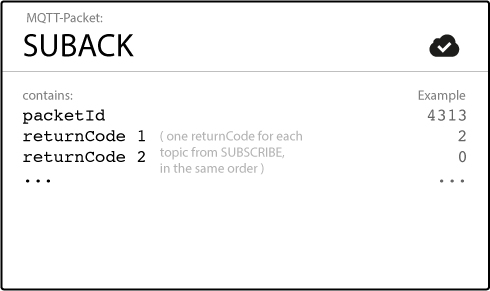
\includegraphics[scale=0.5]{Images/mqtt_suback_message_attributes.png}
	\end{center}
	\legend{Fonte: HiveMQ (2015).}
\end{figure}

Os atributos de uma mensagem do tipo \textit{Suback} são caracterizados abaixo:
\begin{itemize}
	\item packetId: O identificador de pacote identifica exclusivamente uma mensagem;
	\item \textit{Return Code}: O \textit{broker} envia um código de retorno para cada par de tópico/QoS que recebe de mensagens \textit{Subscribe}. O código de retorno reconhece cada tópico e mostra o nível de QoS concedido pelo \textit{broker}. Se o \textit{broker} recusar uma assinatura, a mensagem \textit{Suback} conterá um código de retorno de falha para esse tópico específico.
\end{itemize}

% ----------------------------------------------------------
% Capítulo 2.6.4 - MQTT Unsubscribe Message
% ----------------------------------------------------------
\subsection{MQTT Unsubscribe Message}\label{section_mqtt_unsubscribe_message}
O formato de uma mensagem do tipo \textit{Unsubscribe} está apresentado na \autoref{fig_mqtt_unsubscribe_message_attributes}. A mensagem  \textit{Unsubscribe} é semelhante à mensagem  \textit{Subscribe} e possui um identificador de pacote e uma lista de tópicos.
\begin{figure}[htb]
	\begin{center}
		\caption{Atributos de uma mensagem do tipo \textit{Unsubscribe} para o protocolo MQTT.}\label{fig_mqtt_unsubscribe_message_attributes}
		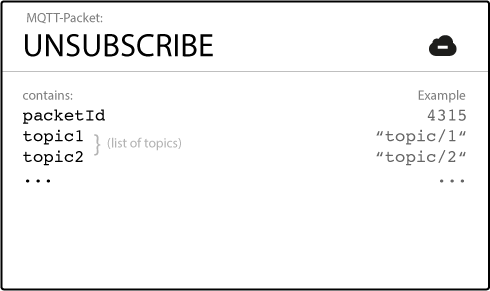
\includegraphics[scale=0.5]{Images/mqtt_unsubscribe_message_attributes.png}
	\end{center}
	\legend{Fonte: HiveMQ (2015).}
\end{figure}

Os atributos de uma mensagem do tipo \textit{Unsubscribe} são caracterizados abaixo:
\begin{itemize}
	\item packetId: O identificador de pacote identifica exclusivamente uma mensagem;
	\item \textit{List of Topic}: A lista de tópicos pode conter vários tópicos dos quais o cliente deseja cancelar a assinatura. Só é necessário enviar o tópico (sem QoS). O \textit{broker} cancela a assinatura do tópico, independentemente do nível de QoS com o qual foi originalmente assinado.
\end{itemize}

% ----------------------------------------------------------
% Capítulo 2.6.5 - MQTT Unsuback Message
% ----------------------------------------------------------
\subsection{MQTT Unsuback Message}\label{section_mqtt_unsuback_message}
O formato de uma mensagem do tipo \textit{Unsuback} está apresentado na \autoref{fig_mqtt_unsuback_message_attributes}. Esta mensagem contém apenas o identificador de pacote da mensagem \textit{Unsubscribe} original.
\begin{figure}[htb]
	\begin{center}
		\caption{Atributos de uma mensagem do tipo \textit{Unsuback} para o protocolo MQTT.}\label{fig_mqtt_unsuback_message_attributes}
		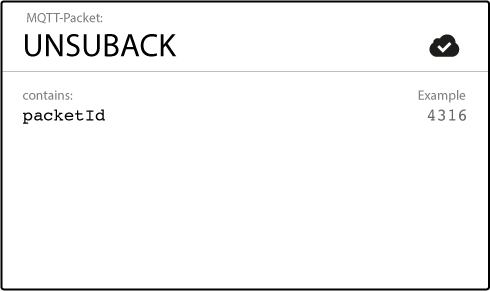
\includegraphics[scale=0.5]{Images/mqtt_unsuback_message_attributes.png}
	\end{center}
	\legend{Fonte: HiveMQ (2015).}
\end{figure}

% ----------------------------------------------------------
% Capítulo 2.3 - Amazon Alexa Voice Service (AVS)
% ----------------------------------------------------------
\section{Amazon Alexa Voice Service (AVS)}
A Amazon Alexa Voice Service é um serviço hospedado em nuvem capaz de integrar diferentes funcionalidades e funções da assistente de voz Alexa em produtos capazes de se conectar à Internet. Esse serviço oferece aos desenvolvedores de dispositivos inteligentes um conjunto de APIs que permitem a integração desses dispositivos com a Alexa. Ao se conectar à Alexa, dispositivos passam a ter acesso a todas as as habilidades da Alexa, também chamadas de \textit{Alexa Skills}. Ademais, o AVR provê aos seus usuários ferramentas de reconhecimento automático de fala (\textit{automatic speech recognition}, ASR) e compreensão de linguagem natural (\textit{natural language understanding}, NLU). A \autoref{fig_logo_alexa} mostra o logo da Amazon Alexa.

\begin{figure}[htb]
	\label{fig_logo_alexa}
	\caption{Logo da Amazon Alexa.}
	\begin{center}
		
\includegraphics[scale=0.7]{Images/logo_amazon_alexa.png}
		\legend{Fonte: Amazon AWS (2022).}
	\end{center}
\end{figure}

Alguns serviços ofertados pela AVS aos desenvolvedores são:
\begin{itemize}
	\item \textit{Alexa Built-in Product (ABI)}: Uma categoria de dispositivos AVS com um conjunto de microfones habilitados para \textit{wake word}, alto-falante e um conjunto principal de recursos e funções do Alexa;
	\item \textit{AVS Device SDK}: Bibliotecas baseadas em C++ que aproveitam as APIs AVS. O AVS Device SDK é uma poderosa ferramenta que permite a rápida integração fr quase todos os recursos e funções do Alexa. Essa SDK É modular e abstrato, fornecendo componentes e APIs personalizáveis.;
	\item \textit{The Alexa APIs}: As interfaces AVS que correspondem à funcionalidade do cliente. Cada interface contém mensagens agrupadas logicamente chamadas diretivas (da nuvem) e eventos (do seu cliente). O AVS também fornece APIs para etapas de implementação como autorização e HTTP/2.
\end{itemize}

A seguir tem-se os casos mais comuns de uso da Alexa e que, a partir de recursos da AVS, agora serão acessíveis em dispositivos com a Alexa integrada:
\begin{itemize}
	\item Configuração e autenticação da Alexa;
	\item Acionamento da Alexa por voz ou toque;
	\item Interrompa o Alexa por voz ou toque;
	\item Transmissão e controle de músicas de vários provedores de serviços de música, como o Spotify;
	\item Sincronização de dispositivos para a audição sincronizada de músicas;
	\item Criação e cancelamento de \textit{timers}, alarmes e lembretes;
	\item Receber, excluir e desativar notificações;
	\item Emparelhar com outros dispositivos através de Bluetooth;
	\item Mantenha contato com chamadas, mensagens e anúncios;
	\item Alternar quaisquer configurações disponíveis;
	\item Saiba quando o Alexa está ouvindo, pensando e respondendo por meio de um sistema de atenção;
\end{itemize}

\section{Trabalhos correlatos}

% ----------------------------------------------------------
% Capítulo 4 - Metodologia
% ----------------------------------------------------------
\chapter{Metodologia}

Dentre os diversos serviços fornecidos pela AWS, o projeto fará uso do AWS IoT Core, serviço de integração da AVS com sistemas IoT. A \autoref{fig_project_diagram} mostra o diagrama de integração do sistema embarcado (dispositivo IoT) à AVS, por meio da tecnologia AWS IoT Core.

\begin{figure}[htb]
	\begin{center}
		\caption{Diagrama de uso dos serviços AWS e da AVS no projeto.}\label{fig_project_diagram}
		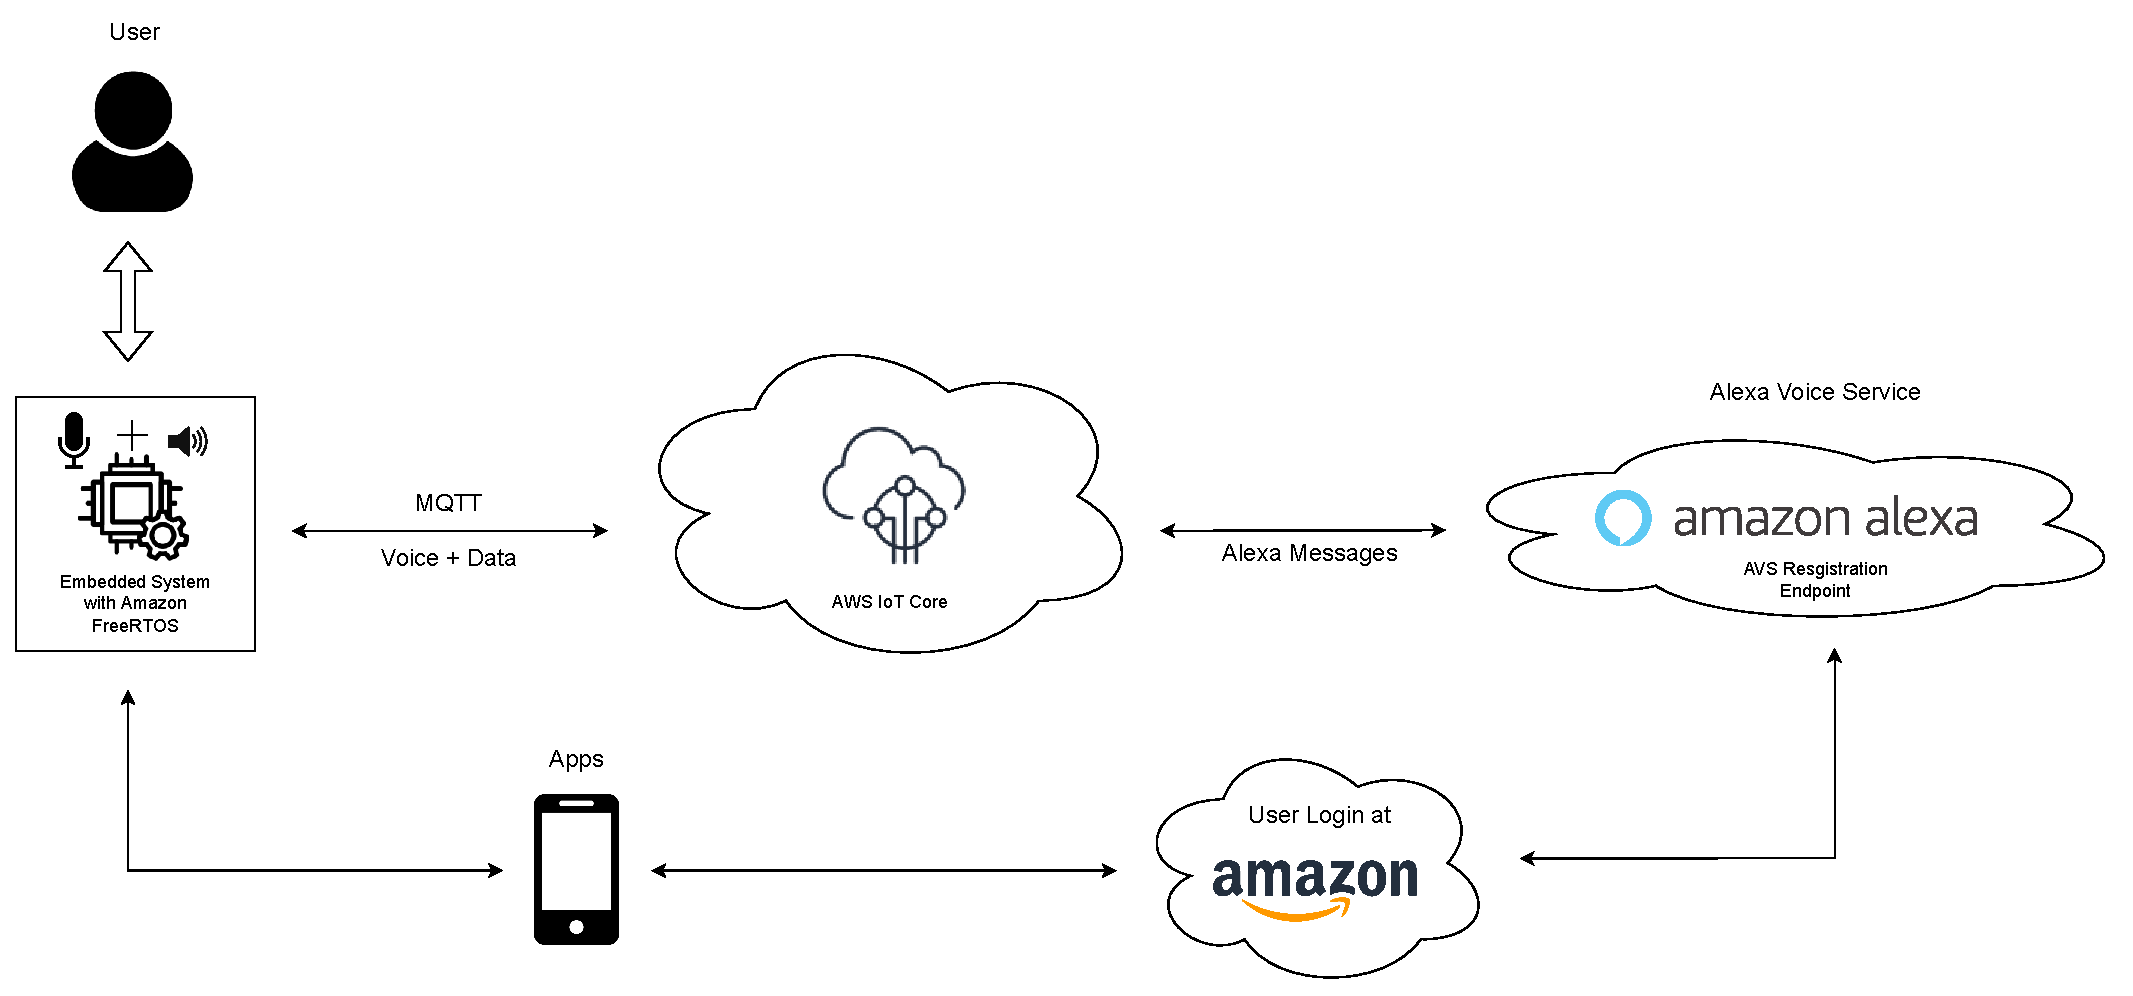
\includegraphics[scale=0.4]{Images/project_diagram.pdf}
	\end{center}
	\legend{Fonte: Autor (2022).}
\end{figure}

\section{Objetivos}
Este trabalho tem o objetivo de criar um sistema embutido de baixo custo integrado aos serviços em nuvem da AWS à assistente de voz Alexa. Para esse dispositivo, tem-se os seguintes requisitos funcionais:
\begin{alineas}
	\item Suporte à rede Wifi IEEE 802.11 (2,4 GHz);
	\item Acionamento da Alexa por voz ou toque;
	\item Comunicação com o usuário em linguagem natural, a partir de caixas de som e microfones;
	\item Ser configurado pelo aplicativo Amazon Alexa;
\end{alineas}

A seguir, tem-se os seguintes requisitos não-funcionais:
\begin{alineas}
	\item Velocidade a definir;
	\item Preço a definir;
	\item Confiabilidade;
	\item Capaz de entender o usuário em ambientes ruidosos (Como medir isso?);
\end{alineas}

\section{Projeto de Hardware}
Para a escolha do hardware do projeto, primeiro estudou-se os requisitos mínimos recomendados pela Amazon. Os parâmetros mínimos recomendados pela AWS podem ser vistos na \autoref{table_reduced_hardware_footprint}.

\begin{table}[]
	\centering
	\begin{tabular}{|c|c|}
	\hline
	\textbf{Processor} & \begin{tabular}[c]{@{}c@{}}ARM M7 or equivalent\\ Arm M4 + AFE DSP\end{tabular} \\ \hline
	\textbf{RAM}       & \begin{tabular}[c]{@{}c@{}}MB for ARM M7\\ 500KB for M4 + AFE DSP\end{tabular}  \\ \hline
	\textbf{Target OS}         & FreeRTOS                      \\ \hline
	\textbf{Connectivity}       & MQTT over Wi-Fi               \\ \hline
	\textbf{\# of Microphones} & 2+                            \\ \hline
	\textbf{Speaker}           & Optimized for speech playback \\ \hline
	\end{tabular}
	\caption{Parâmetros mínimos recomendados pela AWS para o desenvolvimento de um dispositivo de IoT integrado à AVS.}
	\label{table_reduced_hardware_footprint}
	\end{table}

Para a prototipagem, alguns kits de desenvolvimento disponíveis no mercado foram estudados. A \autoref{table_development_kit} mostra uma tabela comparando 4 dispositivos.



% ----------------------------------------------------------
% Capítulo 5 - Resultados e Discussão
% ----------------------------------------------------------
\chapter{Resultados e Discussão}

% ----------------------------------------------------------
% Capítulo 6 - Conclusões
% ----------------------------------------------------------
\chapter{Conclusões}

% ----------------------------------------------------------
% ELEMENTOS PÓS-TEXTUAIS
% ----------------------------------------------------------
\postextual

% ----------------------------------------------------------
% Referências bibliográficas
% ----------------------------------------------------------
\bibliography{abntex2-modelo-references}

\end{document}
